\documentclass[tikz,border=10pt]{standalone}
\usetikzlibrary{arrows.meta}

\begin{document}

{\sffamily

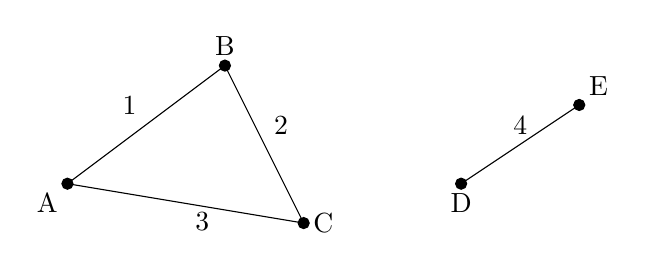
\begin{tikzpicture}

% Triangle component
\filldraw[black] (1,2) circle (2pt) node[below left] {A};  % Node A
\filldraw[black] (3,3.5) circle (2pt) node[above] {B};  % Node B
\filldraw[black] (4,1.5) circle (2pt) node[right] {C};  % Node C

\draw (1,2) -- node[above left] {1} (3,3.5);
\draw (3,3.5) -- node[above right] {2} (4,1.5);
\draw (4,1.5) -- node[below right] {3} (1,2);

% Two-node component
\filldraw[black] (6,2) circle (2pt) node[below] {D};  % Node D
\filldraw[black] (7.5,3) circle (2pt) node[above right] {E};  % Node E

\draw (6,2) -- node[above] {4} (7.5,3);

\end{tikzpicture}

}

\end{document}